\appendix

% NOTE: the System Demonstrations track caps the appendix at 2 pages
% (stricter than the main track). Keep this section tight.

\section{Worked Example: the Verdict Flip}
\label{sec:appendix-example}

The default showcase compares the financial health of Apple (AAPL),
Microsoft (MSFT), and Google (GOOGL): latest ticker info, most recent
quarterly earnings, and one year of price history. The explorer records a
successful trajectory over the \texttt{yfinance} server, which the distiller
compiles into six checkpoints---five tool effects (one carrying a
\{\texttt{download}, \texttt{get\_price\_history}\} equivalence set) and one
value-produced effect over the final message. Table~\ref{tab:agreement} and
the three fixtures of \S\ref{sec:eval} are drawn from this example.

\section{Full-Width Screenshots}
\label{sec:appendix-screenshots}

\begin{figure*}[tbp]
  \centering
  
\includegraphics[width=\textwidth]{figures/fig_studio.png}
  \caption{\textbf{Full-width DMCP Studio screenshot.} Expanded version of
    Figure~\ref{fig:studio}, showing the scoring-stage trajectory, checkpoint
    ledger, Effect/Answer toggle, and editable equivalence-set chip.}
  \label{fig:studio-full}
\end{figure*}

\begin{figure*}[tbp]
  \centering
  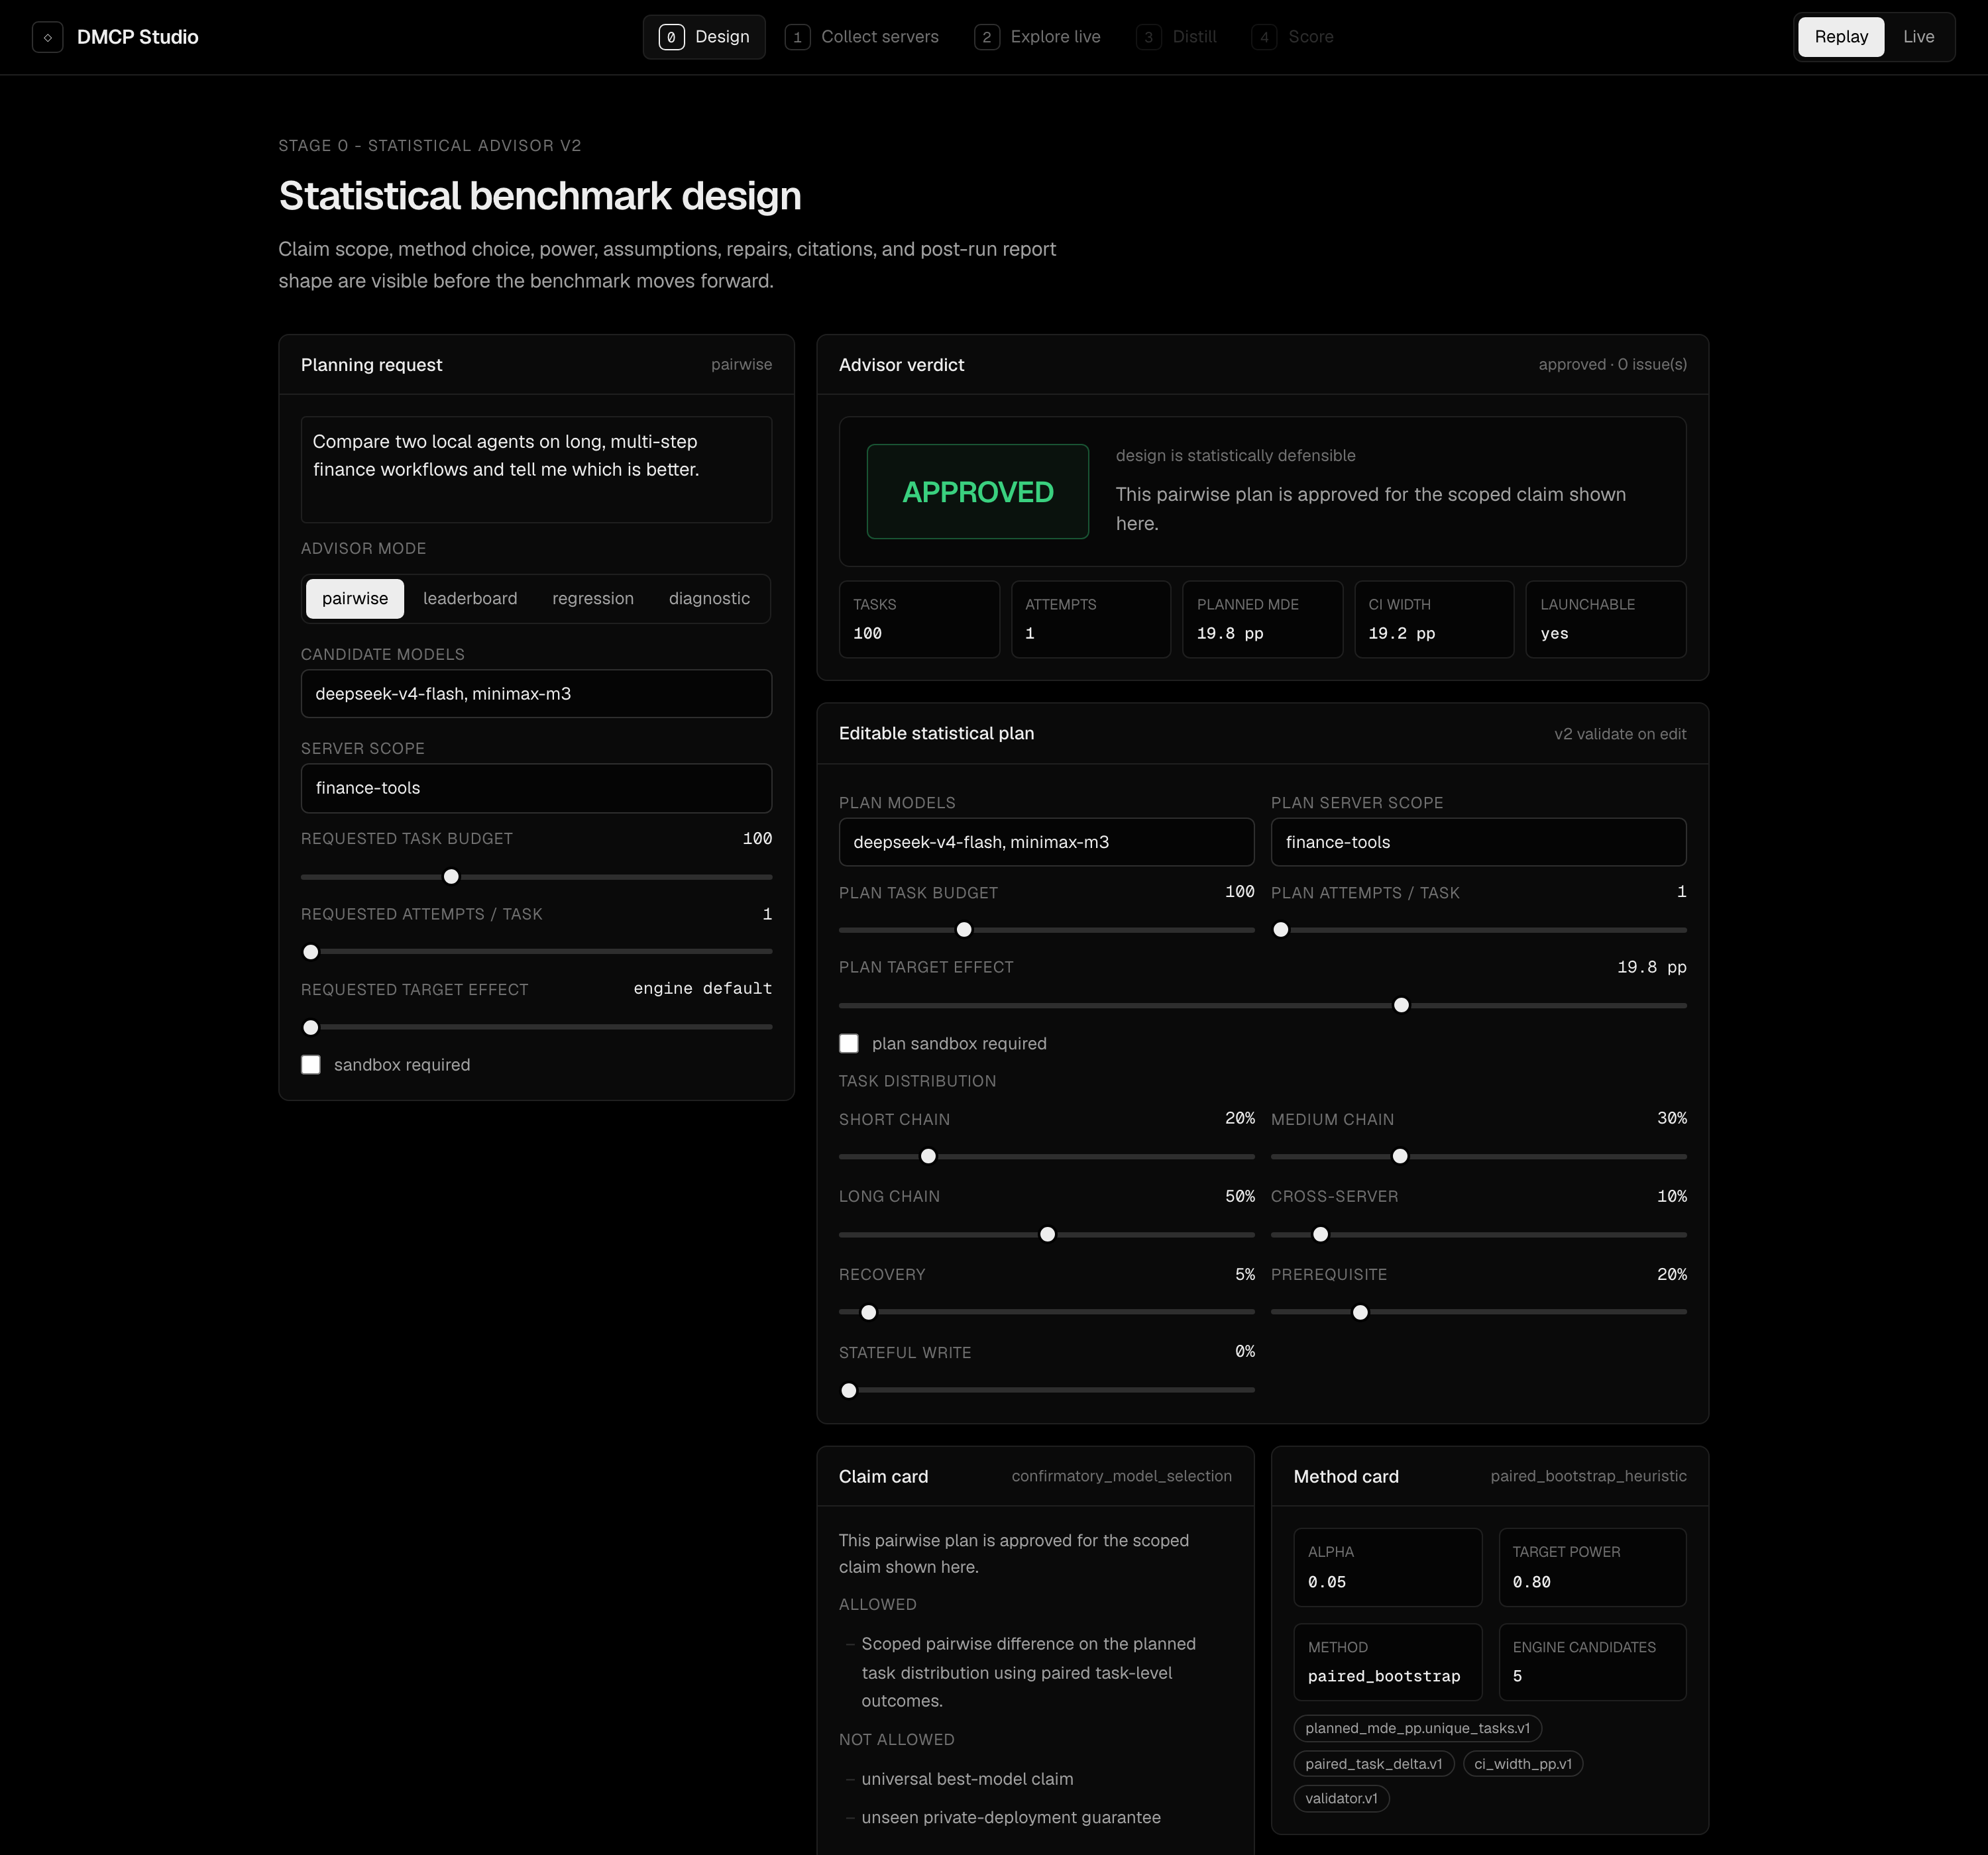
\includegraphics[width=\textwidth]{figures/fig_advisor.png}
  \caption{\textbf{Full-width Benchmark Advisor screenshot.} Expanded version of
    Figure~\ref{fig:advisor}, showing the Stage-0 planning workbench and its
    claim, MDE, assumptions, repairs, alternatives, and guide citations.}
  \label{fig:advisor-full}
\end{figure*}

\section{API Contract}
\label{sec:appendix-api}

The back-end exposes six pipeline routes; \texttt{mode}\,$\in$\,\{\texttt{live},
\texttt{replay}\} defaults to \texttt{replay}. The Stage-0 Benchmark Advisor
adds a parallel \texttt{POST /api/advisor/design}\,/\,\texttt{validate} pair---
and a \texttt{/v2/} statistical-workbench family---that plan and re-validate a
design without touching the pipeline routes below.

\begin{itemize}\itemsep1pt
  \item \texttt{GET /api/servers} --- collected servers with dynamism tags.
  \item \texttt{POST /api/goal} --- generate a goal from a tool surface.
  \item \texttt{GET /api/explore} --- \textbf{SSE} stream of explorer calls.
  \item \texttt{POST /api/distill} --- compile a trace into a TaskSpec.
  \item \texttt{GET /api/score} --- \textbf{SSE} stream of candidate calls
    and per-checkpoint verdicts; the \texttt{done} event returns
    \emph{both} \texttt{effect\_pass} and \texttt{answer\_pass}, so the
    Effect/Answer toggle is a pure front-end re-render.
  \item \texttt{GET /api/leaderboard} --- parent-study results for the peek
    panel (loaded from the real study, never invented).
\end{itemize}
